\section{Estática de los fluidos}

La \textbf{estática de fluidos} es el estudio de fluidos en los que no hay movimiento relativo entre sus partículas. Si no hay movimiento relativo, no existen gradientes de velocidad $\sfrac{du}{dy}$, por lo cual los esfuerzos cortantes serán nulos. El único esfuerzo que existe es un esfuerzo normal, la presión, de modo que ésta tiene la mayor importancia en este estudio.


\subsection{Presión en el seno de los fluidos}%Ver mejor este título

\subsubsection{Presión en un punto}

La presión en un punto de un fluido es constante, es decir, \textsl{la presión es una función escalar y no depende de la dirección normal del área}. Actúa igualmente en todas las direcciones.

\begin{equation}
	p_x = p_y = p_z = p
\end{equation}

%Esta imagen estaba por la demostracion pero me dio paja escribir todo, si quieren saquenla o dejenla, para que se entienda a qué van las p que están arriba...o sea, px py pz
\begin{figure}[H]
	\centering
	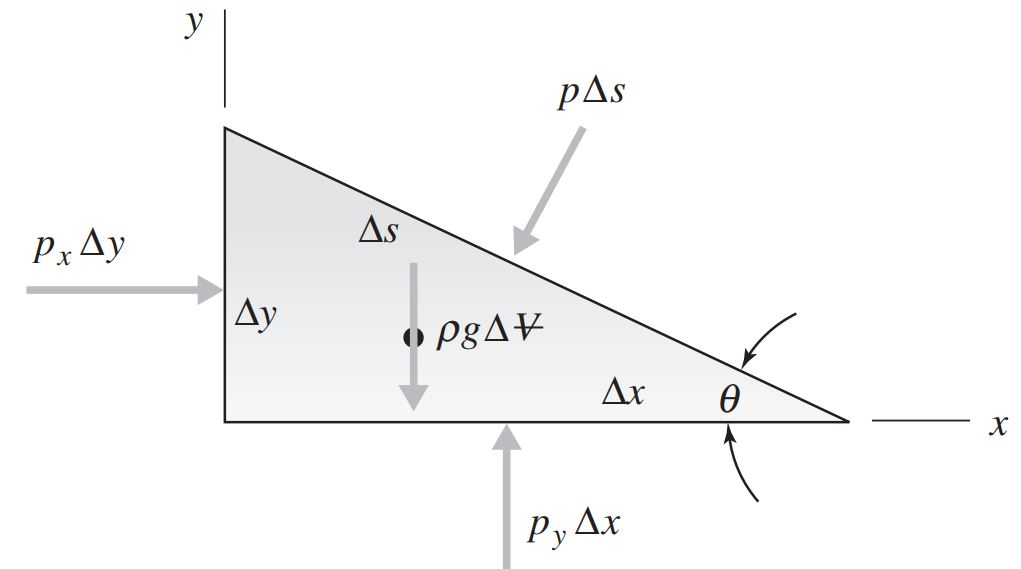
\includegraphics[width = .5 \linewidth]{U2-fluido-infinitesimal}
	\caption{Presión en un punto en un fluido.}
	\label{fig:elemento-infinitesimal}
\end{figure}

\subsubsection{Variación de presión}

%Para determinar la variación de presión de fluidos en reposo, se considera el elemento infinitesimal que se ilustra en la figura \ref{fig:elem-infinitesimal}.
%
%\begin{figure}[H] 
%	\centering
%	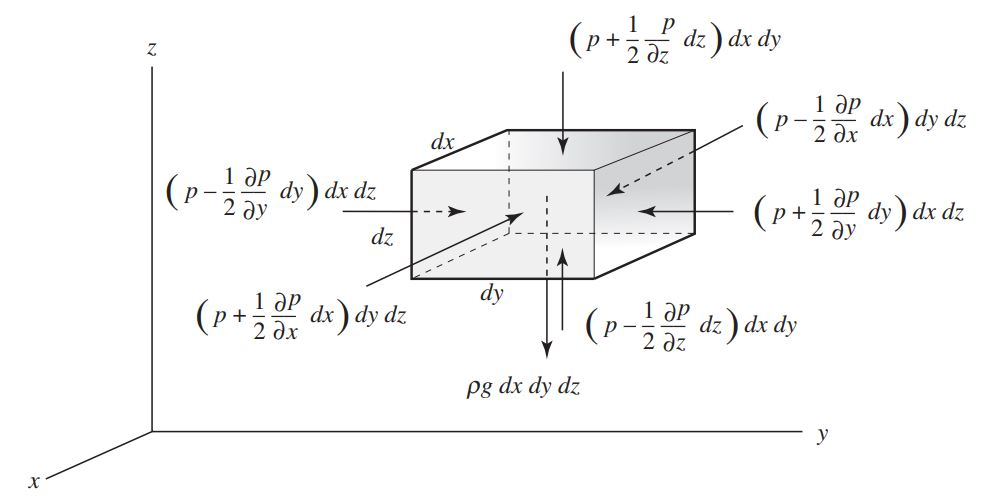
\includegraphics[width = .8\linewidth]{elemento-infinitesimal}
%	\caption{Fuerzas que actúan sobre un elemento infinitesimal de fluido.}
%	\label{fig:elem-infinitesimal}
%\end{figure}
%
%Las presiones en cada uno de los lados se pueden expresar utilizando la \textsl{regla de la cadena} del cálculo infinitesimal con $p\left(x,y,z\right)$:
%
%\begin{equation*}
%	dp = \dfrac{\partial p}{\partial x} dx + \dfrac{\partial p}{\partial y} dy + \dfrac{\partial p}{\partial z} dz
%\end{equation*}
%
%Si nos movemos una distancia $\dfrac{dx}{2}$, la presión será:
%
%\begin{equation*}
%	p\left(x + \dfrac{dx}{2},y,z\right) = p(x,y,z) + \dfrac{\partial p}{\partial x} \dfrac{dx}{2}
%\end{equation*}
%
%Considerando a la Ley de Newton en forma vectorial para un sistema de masa constante como la sumatoria de las fuerzas igualadas a la aceleración por su masa, se llega a tres ecuaciones de componentes:
%
%\begin{align*}
%	-\dfrac{\partial p}{\partial x}\ dx\ dy\ dz & = \rho a_x\ dx\ dy\ dz\\
%	-\dfrac{\partial p}{\partial y}\ dx\ dy\ dz & = \rho a_y\ dx\ dy\ dz\\
%	-\dfrac{\partial p}{\partial z}\ dx\ dy\ dz & = \rho (a_z+g)\ dx\ dy\ dz\\
%\end{align*}

Para determinar la variación de presión de fluidos se utiliza la ecuación \ref{eq:variacion-de-presion} que representa el diferencial de presión en cualquier dirección. 

\begin{equation}
	dp = -\rho a_x dx -\rho a_y dy -\rho (a_z + g) dz
	\label{eq:variacion-de-presion}
\end{equation}

En la estática de fluidos se trabajan con fluidos en reposo, es decir, que no tienen aceleración además de la que experimentan con la aceleración de la gravedad ($a_x = a_y = a_z = 0$).\\


Entonces, para dichos fluidos se llega a la \textbf{ecuación fundamental de la hidrostática}, donde la presión varía en la dirección vertical:

\begin{equation}
	\dfrac{dp}{dz}= - \gamma = - \rho\ g
	\label{eq:fundamental}
\end{equation}

Tambien, tenemos que tener en cuenta que $dp$ se incrementa cuando $dz$ disminuye; esto es, la presión \textbf{aumenta} cuando nos movemos \textbf{hacia abajo} y disminuye cuando es hacia arriba.\\

Si se integra la ecuación \ref{eq:fundamental} se llega a:

\begin{equation}
	P_1 - P_2 = \gamma (z_2 - z_1)
	\label{eq:fundamental-integrada}
\end{equation}\\


Supongamos ahora que se tiene un fluido contenido en un vaso de precipitado como se ilustra en la figura \ref{fig:precipitado}. 

\begin{figure}[H]
	\centering
	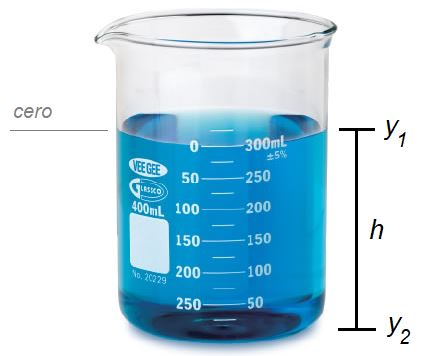
\includegraphics[width = .3\linewidth]{U2-vaso-de-precipitado}
	\caption{Presión en un fluido en reposo}
	\label{fig:precipitado}
\end{figure}

Al estar en contacto con el aire, la presión en el punto 2 será la atmosférica $P_{atm}$, y la ecuación \ref{eq:fundamental-integrada} quedará de la siguiente manera:

%Falta...
\begin{tikzpicture}
	% Ejes cartesianos
	\draw[gray, thick] (0, 0) -- (4, 0) node[right] {$x$};
	\draw[gray, thick] (0,0) -- (0, 4.5) node[right] {$y$};
	
	% Estilo de la función lineal decreciente
	\tikzset{funcion/.style={black, thick}}
	
	% Función lineal decreciente
	\draw[funcion] (1.01325, 4) -- (1.01325+1, 0) node[right] {$P_1(h) = P_{atm} + \gamma\ h$};

	
\end{tikzpicture}



\begin{equation}
	P_1 - P_{atm} = \gamma (z_2 - z_1)
\end{equation}


A la diferencia $P_1 - P_{atm}$ se la denomina como \textbf{presión hidrostática} o manométrica.\\



Si se despeja la presión $P_1$ se llega a la expresión para el \textbf{Segundo Principio de Pascal}:

\begin{equation}
	P_1 = P_{atm} + \gamma h
\end{equation}

\subsection{Manómetros} %Ver este también
Los manómetros son instrumentos que usan columnas de líquidos para medir presiones. Estudiaremos tres tipos, pero todos se basan en la ecuación fundamental de la hidrostática:

\subsubsection{Manómetro de tubo U}
Para medir presiones relativamente pequeñas, usamos un manómetro como se ve en la figura \ref{fig:manometro-u}. Si trazamos una linea horizontal imaginaria que pase por 1, la presión en ambos lados del manómetro será igual. Entonces
\begin{gather}
	P_{1} = P_{1'} \\
	P_{1} = P_{2} + \gamma \, h = P_{atm} + \gamma \, h\\
\end{gather}
Donde $\gamma$ es el peso específico del fluido que se utilize

\begin{figure}[h]
	\centering
	\begin{subfigure}[b]{.45\linewidth}
		\centering
		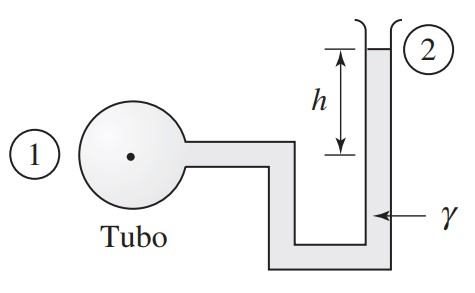
\includegraphics[width = .6\linewidth]{U2-manometro-U}
		\caption{Presiónes pequeñas}
		\label{fig:manometro-u}
	\end{subfigure}
	\begin{subfigure}[b]{.45\linewidth}
		\centering
		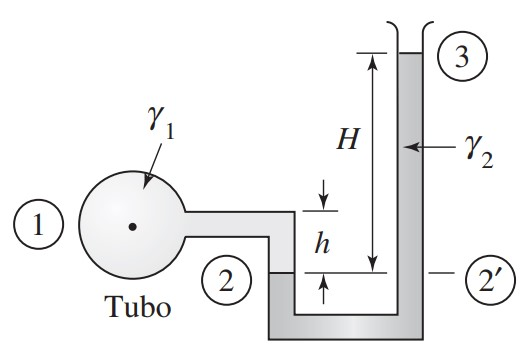
\includegraphics[width = .6\linewidth]{U2-manometro-U1}
		\caption{Presiónes grandes}
		\label{fig:manometro-u2}
	\end{subfigure}
	\caption{Manómetros de tubo en U}
\end{figure}

Cuando necesitemos medir presiones relativamente grandes usamos un manómetro como se ve en la figura \ref{fig:manometro-u2}. Siguiendo la misma metodología que el caso anterior, pero ahora existen dos fluidos no miscibles dentro del tubo.

\begin{gather}
	P_{2} = P_{2'}\\
	P_{1} + \gamma_{1} h = P_{atm} + \gamma_{2} H 
\end{gather}

\subsubsection{Micromanómetro}
Lo usamos para medir cambios de presión muy pequeños. Seguimos con el mismo principio que usamos anteriormente.
\begin{gather}
	P_{3}=P_{3'}\\
	P_{1} + \gamma_{1} (z_{1}-z_{2}) + \gamma_{2} (z_{2}-z_{3}) = P_{5} + \gamma_{2} (z_{5} - z_{4}) + \gamma_{3} (z_{4} - z_{3'})
\end{gather}
Observando que $z_{2}-z_{3} + h = z_{5} - z_{4} + H$
\begin{gather}
	P_{1} = \gamma_{1} (z_{2} - z_{1}) + \gamma_{2} (h- H) + \gamma_{3} \\
	P_{1} = \gamma_{1} (z_{2} - z_{1}) + \gamma_{2} h + (\gamma_{3} -\gamma_{2}) H
\end{gather}

\begin{figure}[h]
	\centering
	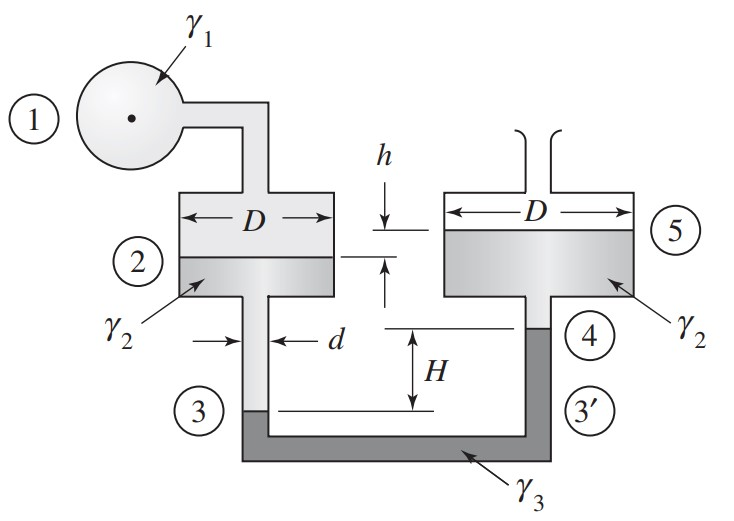
\includegraphics[width = .4\linewidth]{U2-micromanometro}
	\caption{Micromanómetro}
	\label{fig:micro}
\end{figure}
\subsubsection{Efecto de la fuerza superficial sobre un fluido confinado}
Si se ejerce una presión externa sobre una parte de la frontera de un fluido confinado, esta presión se transmite uniformemente a través de todo el fluido.
\\
Este principio explica el funcionamiento de gatos hidráulicos, prensas, frenos, y diversos mecanismos que transmiten fuerzas a través de un fluido.


\begin{figure}[h]	
	\centering
	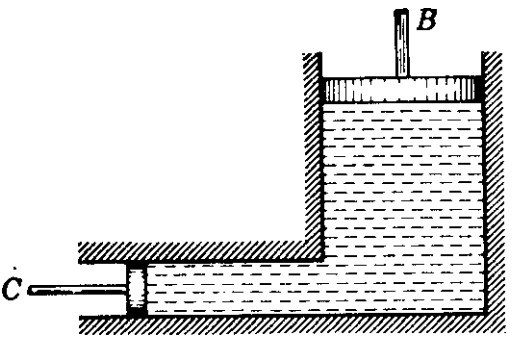
\includegraphics[width = .2\linewidth]{U2-gato-hidraulico}
	\caption{Gato hidráulico}
	\label{fig:gato}
\end{figure}

\begin{equation}
	\dfrac{F_{B}}{F_{C}} = \dfrac{\Delta P A_{B}}{\Delta P A_{C}} = \dfrac{A_{B}}{A_{C}}
\end{equation}


\subsection{Fuerzas sobre superficies}
\subsubsection{Planas}
Si sumergimos una placa plana, sobre ésta actuara una presión constante (sobre la superficie libre) y una presión causada por la gravedad que se incrementa uniformemente.
\begin{figure}[h]
	\centering
	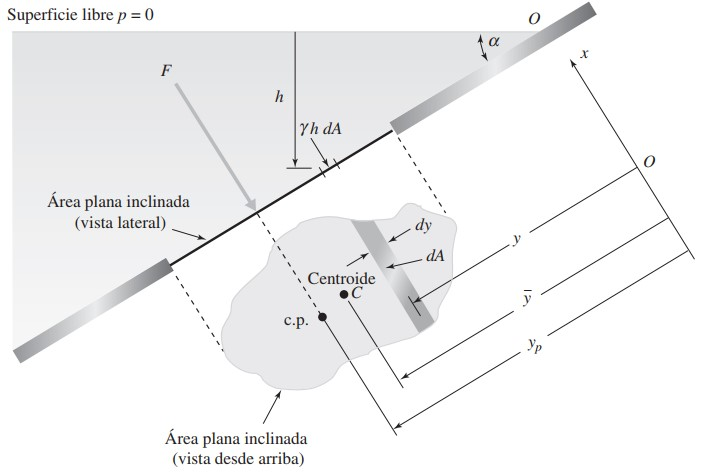
\includegraphics[width = .6\linewidth]{U2-sup-plana}
	\caption{Fuerza sobre área plana}
	\label{fig:sup-plana}
\end{figure}
Debido a que no puede existir esfuerzo cortante, esta fuerza debe ser perpendicular a la superficie sumergida. Observando la figura \ref{fig:sup-plana}, sobre el elemento \textbf{dA} actúa una presión constante. La magnitud de la fuerza sobre este elemento será $\gamma \, h \, dA$. Si integramos sobre el área completa de la placa
\begin{equation*}
	F = \int_{A} \gamma \ h \ dA = \int_{A} \gamma \ y \sin \theta \ dA =  \gamma \sin \theta \int_{A} y \ dA
\end{equation*}
La integral que queda es el primer momento de \emph{área} de la placa con respecto al eje \emph{x}; esto es equivalente a usar \textbf{$A \ \overline{y}$}, doonde $\overline{y}$ es la distancia al centroide de la superficie. Entonces la magnitud de la fuerza, teniendo en cuenta la presion en la superficie libre será:

\begin{equation}
	F =(P_{s} + \overline{y} \sin \theta \ \gamma) A
\end{equation}

Como la fuerza resultante no actúa en el centroide de la placa, para hallar la ubicación de esta igualamos la suma de los momentos de todas las fuerzas de presión que actúan sobre el área con el momento generado por la fuerza misma. Si la fuerza F actúa en el punto $(x_{p}, y_{p})$:

\begin{equation*}
	y_{p} F = \int_{A} y (P_{s} \overline{y} \sin \theta \ \gamma ) dA
\end{equation*}

Desarrollando llegamos a la siguiente ecuación:

\begin{equation}
	y_{p} = \overline{y} + \dfrac{\overline{I}_{x}}{A \overline{y}}
\end{equation}

Donde $\overline{I}_{x}$ es el momento de inercia centroidal de la placa respecto de $x$.
\\
De igual manera para hallar la coordenada $x_{p}$
\begin{equation*}
	x_{p} F = \int_{A} y (P_{s} \ \overline{y} \ \sin \ \theta \ \gamma ) dA
\end{equation*}
\begin{equation}
	x_{p} = \overline{x} + \dfrac{\overline{I}_{xy}}{A \overline{y}}
\end{equation}
Donde $\overline{I}_{xy}$ es el producto de inercia centroidal y $\overline{x}$ la distancia al eje $y$ centroidal.

\subsubsection{Curvas}
En este tipo de casos, no se utiliza un método directo para llegar al resultado, sino que se realiza un diagrama de cuerpo libre en el cual mediante integración se van determinando las fuerzas actuantes y ellas nos permitirán plantear las ecuaciones para los resultados.
\begin{figure}[h]
	\centering
	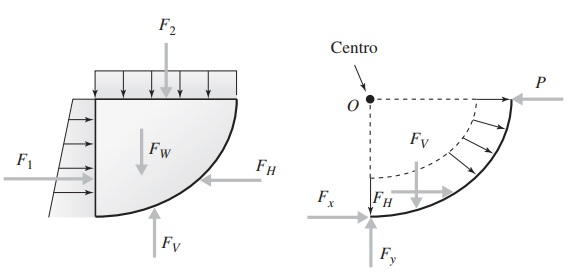
\includegraphics[width = .6\linewidth]{U2-curvas.jpg}
	\caption{Fuerza sobre superficies curvas}
	\label{fig:fuerz-sup-curv}
\end{figure}
Dicho DCL muestra las fuerzas debidas: al agua sobre la curva, $F_{1}$ y $F_{2}$ resultantes ubicadas debido a la distribución de las mismas y $F_{w}$ que es el agua del cuerpo inscripto en la figura. $F_{H}$ y $F_{V}$ son fuerzas que componen las reacciones y que mantienen el equilibrio en el sistema.\\
En este tipo de problemas la llave de la cuestión esta en hallar correctamente donde se encuentra esa fuerza $F_{w}$, que es simplemente el peso de la columna prismática total del fluido que se encuentra por encima de la superficie curva. Si se quiere tener en cuenta la presión sobre la superficie solo se le suma a $F_{w}$ el producto entre $p_{s}$ y el área proyectada de la superficie curva vista desde arriba.

Conociendo ello solo basta plantear sumatoria de momentos respecto al vínculo de grado 2 de la compuerta.

\subsection{Cuerpos sumergidos}
\subsubsection{Empuje de flotación}
El \textbf{Princípio de Arquímedes} establece que la fuerza de flotación que aparece en un cuerpo sumergido es igual al peso del volumen de líquido desplazado.\\
También conocida como fuerza de boyamiento, resultante ejercida sobre un cuerpo por un fluido estático que se encuentra sumergido o flotando, esta fuerza siempre actúa verticalmente.
\begin{equation}
	F_{B}=\gamma V_{\text{líquido desplazado}}
	\label{ec:fuerz-boy}
\end{equation}
Donde esta fuerza de boyamiento actuará en el centroide del volumen desplazado. En líquidos compresibles no será asi ya que $\gamma$ depende de $z$.

\subsubsection{Estabilidad de flotación}
La \textbf{estabilidad vertical} la vemos cuando un objeto encuentra equilibrio entre el peso y la fuerza de boyamiento, cuando se lo quita del equilibrio (hundiendolo/removiendolo) aparecen fuerzas restauradoras que contribuyen a reponer el cuerpo nuevamente al equilibrio.\\
La \textbf{estabilidad rotacional} de un cuerpo sumergido.

\begin{figure}[!h]
	\centering
	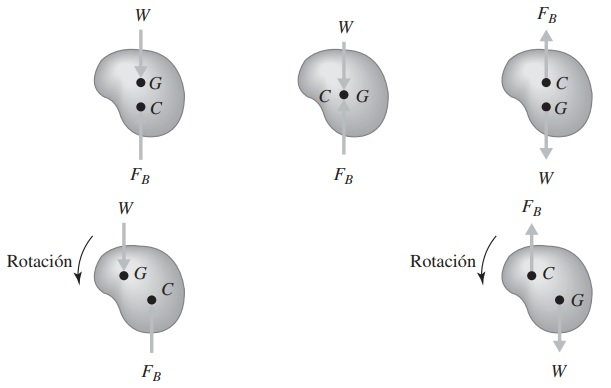
\includegraphics[width = .6\linewidth]{U2-estabilidad2.jpg}
	\caption{Estabilidad cuerpo sumergido}
	\label{fig:est-cuerp-sum}
\end{figure}


Para esto precisamos conocer el concepto de centro de flotabilidad $\textbf{C}$, que no es mas que el punto por el cual pasa la resultante de la fuerza de boyamiento.\\
Un análisis rápido nos que nos dará criterio para estabilidad depende de las posiciones relativas \textit{(cuál se encuentra arriba)}:\\
\begin{tabular}{p{\textwidth}}
	$\bullet$ $\textbf{G}$ arriba de $\textbf{C}$ una pequeña rotación angular resulta en un momento que continuará aumentando la rotación, \textbf{No estable}\\
	$\bullet$ $\textbf{G}$ sobre  $\textbf{C}$ neutral\\
	$\bullet$ $\textbf{G}$ abajo de $\textbf{C}$ una pequeña rotación angular resulta en un momento restaurador, \textbf{Estable}\\
\end{tabular}\\

Sin embargo un cuerpo puede ser estable aun si $\textbf{G}$ está por encima de $\textbf{C}$ en el caso de cuerpos en flotación. Observando la figura \ref{fig:sec-transv} cuando el cuerpo gira el centroide $\textbf{C}$ se mueve a $\textbf{C'}$, y si $\textbf{C'}$ se traslada lo suficientemente lejos puede desarrollar un momento restaurador y el cuerpo es estable.\\
En este tipo de situaciónes lo que hay que analizar es el valor de la \textbf{altura metacéntrica $\widehat{GM}$}, definida como la distancia de G al punto de intersección de la fuerza de flotación antes de la rotación con la fuerza de flotación despues de la rotación:\\
\begin{tabular}{p{\textwidth}}
	$\bullet$ $\widehat{GM}>0$ cuerpo estable.\\
	$\bullet$ $\widehat{GM}<0$ cuerpo inestable.
\end{tabular}\\
\begin{figure}[!h]
	\centering
	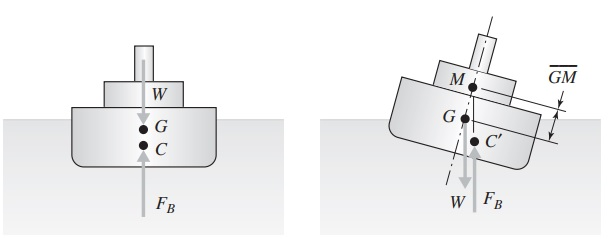
\includegraphics[width = .6\linewidth]{U2-estabilidad3.jpg}
	\caption{Sección transversal cuerpo en flotación}
	\label{fig:sec-transv}
\end{figure}
\begin{multicols}{2}
	\begin{tabular}{c}
		El valor de $\widehat{GM}$ se puede calcular como\\
		$\widehat{GM}=\dfrac{I_{o}}{V_{desplazado}}-\widehat{CG}$\\
	\end{tabular}
	\begin{tabular}{c}
		El valor del momento restaurador:\\
		$C=\gamma~ \Delta \theta~ I_{yy}$\\
	\end{tabular}
\end{multicols}

\subsection{Equilibrio relativo}

\subsubsection{Aceleración lineal uniforme}	
El fluido se encuentra en reposo con relación a un marco de referencia acelerado en \emph{x} e \emph{y}. Recordando la ecuación \ref{eq:variacion-de-presion}, esta se simplifica a:
\begin{equation}
	dp = - \rho a_{x} dx - \rho(g + a_{z}) dz
\end{equation} 

Integrando entre los puntos 1 y 2 tenemos:

\begin{equation}
	p_{2}- p_{1} = - \rho a_{x}(x_{2}-x_{1}) - \rho(g + a_{z}) (z_{2}-z_{1})
\end{equation}
\begin{figure}[h]
	\centering
	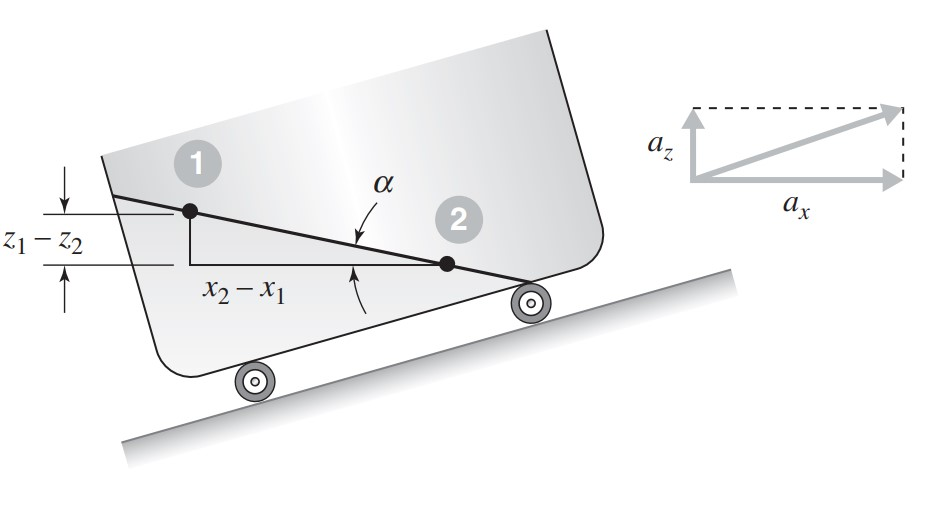
\includegraphics[width = .5\linewidth]{U2-aceleracion-lineal}
	\caption{Depósito linealmente acelerado}
\end{figure}

Si los puntos 1 y 2 se encuentran a la misma presión entonces:
\begin{equation}
	\dfrac{z_{1}-z_{2}}{x_{2}-x_{1}} = \tan \alpha = \dfrac{a_{x}}{g-a_{z}}
\end{equation}
\\
\subsubsection{Rotacion uniforme alrededor de un eje vertical}

La ecuacion diferencial de presion:
\begin{equation}
	dp = \rho r \omega^{2} dr - \rho g dz
\end{equation}
Si elegimos el centro de coordenadas en el vértice del paraboloide e integramos la ecuación.
\begin{equation}
	p -p_{0} = \dfrac{\rho \omega^{2} }{2} r^{2} - \rho g z
\end{equation}
\begin{figure}[h]
	\centering
	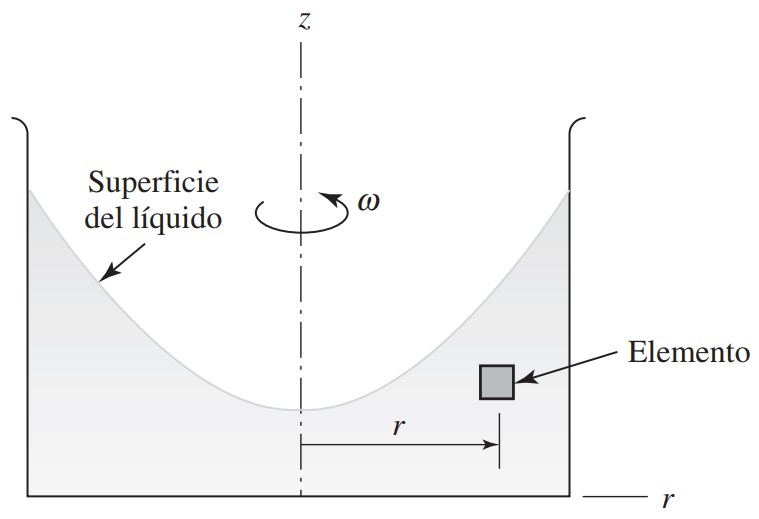
\includegraphics[width = .4\linewidth]{U2-rotacion-uniforme}
	\caption{Depósito sometido a rotación}
\end{figure}
Si los dos puntos considerados se encuentran a la misma presión como la superficie libre entonces $p - p_{0} = 0$ y nos queda una ecuación de una parábola que corta el origen:

\begin{equation}
	z = \dfrac{\omega^{2} r^{2} }{2 g}
\end{equation}

El origen de coordenadas se puede encontrar igualando el volumen del fluido en reposo y cuando se encuentra en rotación uniforme.